% #####################################################################
\chapter{Background}\label{chap:fundamentacao}
% #####################################################################

% =====================================================================
\section{MIMO System}\label{sec:sistemas-MIMO}
% =====================================================================
A cellular network consists of a set of Base Stations (BSs) and a set of User Equipment (UEs). Each EU is served by a base station. The downlink is the transmission from the BSs to their UEs, and the uplink is the transmission from the UEs to their BS. The area served by a BS is its cell \cite[pp.~7--8]{bjornson-mimo}. \textcolor{blue}{The wireless access technology in fifth-generation (5G) cellular networks is New Radio (NR) \cite[p.~2]{lin-lee-5g}.} It operates in two frequency bands: FR1 (Frequency Range 1), from 410 MHz to 7125 MHz, and FR2, from 24250 MHz to 52600 MHz \cite[Tab.~5.1-1]{3gpp-ts38104}.

In a massive multi-input multiple-output (MIMO) system, the BS has $M$ antennas and serves $K$ UEs, each with one antenna (Figure \ref{fig:uplink-mimo}). All UEs use the same time and frequency resources simultaneously, and the BS needs to separate the signal from each one, received by each antenna of the Base Station into its own RF chain. The number of antennas $M$ is usually much greater than $K$, and only the BS knows the channel \cite[p.~11]{marzetta2016fundamentals}. \textcolor{blue}{The BS in this work has $M = 128$ or 256 antennas, as in \cite{zhao2025jsac}.}


% FONTE: decentralized2017, p. 492.


\begin{figure}[!ht]
\caption{Uplink of a massive MIMO system: $K$ single-antenna UEs and a BS with $M$ antennas.}
\label{fig:uplink-mimo}
\vspace{4pt}
\centering
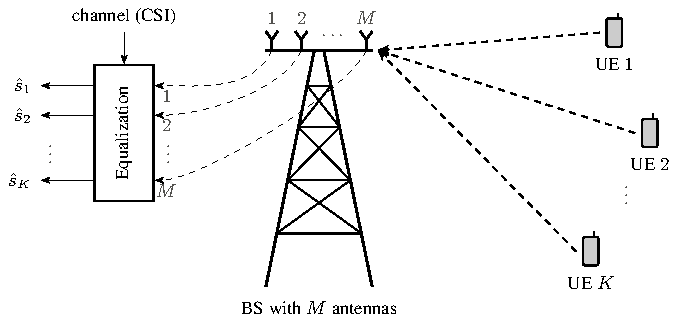
\includegraphics{Images/FLUXO/uplink_mimo.pdf}
\vspace{4pt}
\legend{Source: adapted from \citesp{marzetta2016fundamentals}, p.~12.}
\end{figure}

% FONTE: Marzetta et al. 2016, Seção 1.3, pp. 10-11; Björnson et al. 2017, p. 349; M = 128 ou 256: zhao2025jsac paper.md:577.
% FONTE: Björnson et al. 2017, pp. 7-8 (Fig. 1.1) e p. 30; Marzetta et al. 2016, p. 11 e Fig. 1.4(a), p. 12 (adaptada).

\subsection{Uplink}\label{subsec:uplink}
% FONTE: TG1 (sbc-template.tex), Uplink System Model.
The uplink data transmission
can be modeled by:

\begin{equation}
\mathbf{y} = \mathbf{H}\mathbf{s} + \mathbf{n}
\label{eq:systemmodel}
\end{equation}
where $\mathbf{y} \in \mathbb{C}^{M\times1}$ is the vector of signals received at the
antennas of the BS, $\mathbf{s} \in \mathbb{C}^{K\times1}$ is the vector of
symbols transmitted by the $K$ users, $\mathbf{H} \in \mathbb{C}^{M\times K}$
is the channel matrix, and $\mathbf{n}$ represents the noise vector
received at the BS~\cite{rodriguezsanchez2020}.

Each received element $y_m$ corresponds to the linear combination of the $K$ symbols
transmitted by all users, weighted by the coefficients of the channel matrix $\mathbf{H}$ of antenna $m$, plus the noise contribution $n_m$.

\textcolor{blue}{The baseband processing of the uplink in the BS has several tasks: converting signals between time and frequency domains, compensating for signal imperfections, recovering symbols, and detecting the data, which is then decoded \cite{decentralized2017}.}

To recover the symbols, BS combines the signals from all antennas. The various antennas only provide gain when BS knows the channel response of each UE, because this knowledge allows combining the signals coherently \textcolor{red}{\cite{bjornson-mimo}}. This step is equalization (Figure). \textcolor{blue}{The detection stage then transforms the received symbols into bits according to the adopted encoding.} The goal of equalization is to estimate the vector $\mathbf{s}$ from $\mathbf{y}$ minimizing the detection error.

% ---------------------------------------------------------------------
\subsection{Decentralized Uplink}\label{subsec:dbp}
% ---------------------------------------------------------------------

% FONTE: TG1 (sbc-template.tex), Decentralized MIMO Architectures.
The complexity of estimating the vector s grows with the number of antennas and poses a challenge for the MIMO system \cite{jeon2019}. \textcolor{blue}{The Decentralized Baseband Processing (DBP) architecture was introduced in~\cite{decentralized2017, bertilsson2018distributed} to address this issue.} In DBP, the $M$ base-station antennas are partitioned into $C$ clusters with $M_c$ antennas, each cluster with a Distributed Unit (DU) with local radio-frequency circuitry and baseband processing fabric such as custom ASICs, FPGAs, or DSPs \cite{decentralized2017}. 

The uplink system model for a $C$ cluster becomes:

\begin{equation}
    \mathbf{y}_c = \mathbf{H}_c\mathbf{s} + \mathbf{n}_c,
\end{equation}
where $\mathbf{y}_c \in \mathbb{C}^{M_c \times 1}$,
$\mathbf{H}_c \in \mathbb{C}^{M_c \times K}$, and $\mathbf{n}_c$ is the
local noise vector, with ~\cite{jeon2019}:

\begin{equation}
M = \sum_{c=1}^{C} M_c    
\end{equation}

There are two main topologies for the DBP: star, in which all DUs are connected to a central unit (CU), and daisy-chain, in which the DUs are connected in series via unidirectional links and pass intermediate data along  \cite{rodriguezsanchez2020,zhao2025jsac}. This work employs a daisy-chain topology.
% FONTE: zhao2025jsac paper.md:87-89 e :367; rodriguezsanchez2020 L167.

\subsection{Symbols (\texorpdfstring{$\mathbf s$}{s})}\label{subsec:simbolos}
A symbol represents a group of bits. Modulation defines how each group of bits is converted into a symbol \cite{goldsmith}. In 5G NR, symbols are transmitted within a resource grid, which is formed by subcarriers in the frequency domain and OFDM symbols in the time domain \cite{3gpp-ts38211}.
% FONTE: Goldsmith, p. 127 e pp. 141-142; TS 38.211 v18.6.0, Sec. 4.4.2.

\subsubsection{Modulation}\label{subsubsec:modulacao}
Information bits undergo digital modulation to be transformed into a signal that can be transmitted over a channel. Each group of bits is represented as a point on the complex plane, with an in-phase and a quadrature component. Each point is a symbol, and the set of all such points is called a constellation. In QAM (Quadrature Amplitude Modulation), information is encoded in both amplitude and phase, whereas in PSK (Phase-Shift Keying) it is encoded solely in the phase \cite{goldsmith}.
% FONTE: Goldsmith, p. 127 e pp. 141-142.

The number of points in a constellation determines how many bits each symbol carries. The modulation schemes used in this work, QPSK (Quadrature Phase-Shift Keying) and 16-QAM, have 4 and 16 points, respectively, and carry 2 and 4 bits per symbol (Figure~\ref{fig:constelacoes}). Each symbol is transmitted with an average energy $E_s$ \cite{zhao2025jsac}. The error probability depends on the minimum distance between the points. With the same energy, the points of 16-QAM are closer to each other, so 16-QAM needs a higher SNR than QPSK for the same error probability \cite{tse-viswanath}.
% FONTE: tse-viswanath p. 56 (Eq. 3.24), p. 57 (Fig. 3.3), p. 60 (Tab. 3.1), p. 386 (Eq. 9.12).

\begin{figure}[!ht]
\caption{QPSK and 16-QAM constellations with the same average energy per symbol and the bits of each point.}
\label{fig:constelacoes}
\vspace{4pt}
\centering
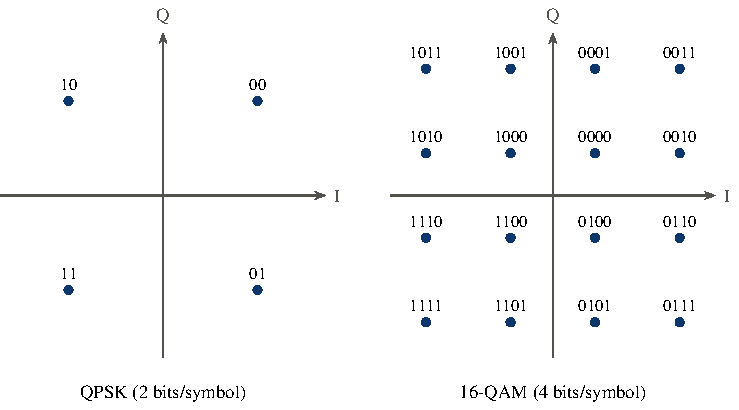
\includegraphics{Images/FLUXO/constelacoes.pdf}
\vspace{4pt}
\legend{Source: adapted from \citesp{goldsmith} and \citesp{3gpp-ts38211}.}
\end{figure}
% FONTE: Goldsmith, Fig. 5.18, p. 149; Tse e Viswanath, p. 57 (Fig. 3.3); TS 38.211 v18.6.0, Secs. 5.1.3 e 5.1.4.

\subsubsection{Resource Grid}\label{subsubsec:grade-recursos}
\textcolor{blue}{These symbols are transmitted in 5G NR using Orthogonal Frequency Division Multiplexing (OFDM), a transmission technique that divides the frequency band into orthogonal subcarriers, each carrying one symbol \cite{tse-viswanath}.} A Resource Element (RE) is one subcarrier during one OFDM symbol. A Resource Block (RB) consists of 12 consecutive subcarriers. The Physical Resource Blocks (PRBs) are the RBs inside the part of the band configured for the transmission, which has from 1 to 275 RBs \cite{3gpp-ts38211, lin-lee-5g}. The number of PRBs in a transmission is denoted as $N_{\text{PRB}}$. Since the receiver processes each PRB, $N_{\text{PRB}} = 275$ is the worst case for 5G NR \cite{zhao2025jsac}.
% FONTE: Tse e Viswanath, Seção 3.4.4, p. 99; TS 38.211 Secs. 4.4.3, 4.4.4.1 e 4.4.4.4; Lin e Lee, p. 367; zhao2025jsac paper.md:640.

In the time domain, OFDM symbols are grouped into slots, each containing 14 symbols. The data of the User Equipments (UEs) is transmitted on the Physical Uplink Shared Channel (PUSCH) \cite{3gpp-ts38211}. A UE transmits the PUSCH only in the slots that the base station assigns to it. In Time Division Duplex (TDD), the uplink and the downlink use the same frequency band, but at different times \cite{lin-lee-5g}. \textcolor{blue}{Therefore, only the uplink slots can carry the PUSCH in TDD.}
% FONTE: Lin e Lee, pp. 104 e 293; TS 38.211 Tab. 4.3.2-1 e Sec. 6.3.1.


\subsection{Channel (\texorpdfstring{$\mathbf H$}{H})}\label{subsec:canal}\label{subsubsec:multipercurso}


The signal transmitted by a UE $k$ to each of the $M$ receiving antennas travels along multiple paths, during which it is subject to constructive and destructive interference. This phenomenon is known as small-scale fading and occurs over distances on the order of the signal's wavelength. \textcolor{blue}{The result is large-scale fading when path loss and shadowing, caused by large obstacles such as buildings or hills, are also taken into account \cite{tse-viswanath}.}

The channel matrix $\mathbf{H}$ models the attenuation, fading, and phase shifts of the signals between the UEs and the BS \cite{rodriguezsanchez2020}. Column $k$ represents the channel gains between UE $k$ and each of the $M$ antennas \cite{tse-viswanath}.
% FONTE: rodriguezsanchez2020; Tse e Viswanath, Seção 7.2, Eq. 7.18, p. 297.

\subsubsection{Coherence Time}\label{subsubsec:tempo-coerencia}
As a user moves, the received signal undergoes a Doppler shift, causing variations in the communication channel. The greater the Doppler shift, the shorter the time interval during which the channel can be considered approximately constant. This interval is known as the coherence time ($T_c$) and is calculated based on the maximum Doppler shift ($f_D$) \cite{tse-viswanath}. \textcolor{blue}{The coherence time values in this work are determined using the $f_D$ values specified in the test conditions established by 3GPP \cite{3gpp-ts38104} for the FR1 and FR2 frequency ranges.}
% FONTE: Tse e Viswanath, pp. 10, 13, 30-31 (Eq. 2.44) e 70 (v = f_D c / f_c).
%   f_D: TS 38.104 v16.4.0, Anexo G, Tabs. G.2.2-1, G.2.2-2, G.3-1 e G.3-2; f_c: TS 38.104 Tabs. 5.2-1 e 5.2-2.
%   Mobilidade: ITU-R M.2083-0, pp. 4, 11, 14 e 15. Valores: software/Restrições - Parâmetros.csv, linhas 15-24.

\subsubsection{Coherence Block}\label{subsec:bloco-coerencia}
The frequency interval over which the channel remains approximately constant is called the Coherence Bandwidth ($B_c$). A coherence block is a region with duration $T_c$ and bandwidth $B_c$. Within the coherence block, the effect of the channel on the signal is the same as multiplying by a complex gain \cite{marzetta2016fundamentals} (Figure~\ref{fig:bloco-coerencia}). \textcolor{blue}{This work uses $B_c = 1$ PRB \cite{zhao2025jsac}.}
The number of OFDM symbols in a coherence block is limited by $T_c$. \textcolor{blue}{Table~\ref{tab:n-maximo} shows how many OFDM symbols fit within $T_c$ for each test condition, with subcarrier spacings of 30 kHz (FR1) and 120 kHz (FR2) \cite{3gpp-ts38104}.}

% FONTE: SCS: TS 38.104 Tab. 5.3.5-1 (n78) e 5.3.5-2 (n257).
% FONTE: Marzetta et al., Seções 2.1.2 e 2.1.3, pp. 21-22.
\begin{figure}[!ht]
\caption{Time-frequency plane divided into coherence blocks.}
\label{fig:bloco-coerencia}
\vspace{4pt}
\centering
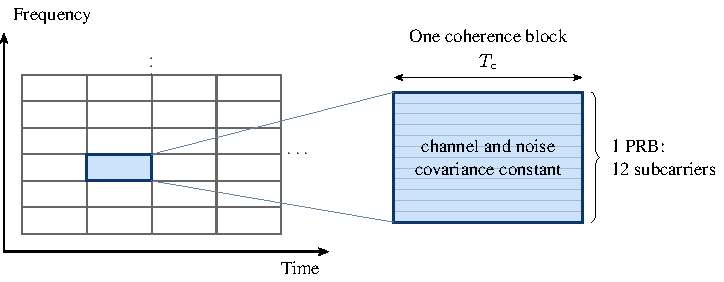
\includegraphics{Images/FLUXO/bloco_coerencia.pdf}
\vspace{4pt}
\legend{Source: adapted from \citesp{bjornson-mimo}.}
\end{figure}
% FONTE: zhao2025jsac (canal constante no PRB). Figura: Björnson et al., Fig. 2.1, p. 67.



\subsection{Colored Noise (\texorpdfstring{$\mathbf n$}{n})}\label{subsec:interferencia}
The BS receives signals from the $K$ UEs it serves (target UEs), whose symbols form the vector $\mathbf s$. Signals received from non-target UEs interfere with data reception and are treated as noise. These signals, together with thermal noise, form the vector $\mathbf n$ in Equation~\ref{eq:systemmodel}. The interference makes the covariance matrix of $\mathbf n$ non-diagonal, and for this reason $\mathbf n$ is called colored noise \cite{zhao2025jsac}.
% FONTE: zhao2025jsac paper.md:33, 108-113, 577.

\subsubsection{Thermal Noise}\label{subsubsec:ruido-termico}
Thermal noise arises from the random motion of electrons in the conductors and devices of the receiver front end. This noise is modeled as additive white Gaussian noise (AWGN), which has a Gaussian distribution with zero mean and the same power spectral density at all frequencies \cite{haykin,tse-viswanath}. The noise at the $M$ antennas is described by an $M \times M$ covariance matrix, in which each element is the correlation between the noise of a pair of antennas. Thermal noise is independent at each antenna, so only the diagonal elements of this matrix are non-zero. Each diagonal element is the average thermal noise power at one antenna, $\sigma^2$, and the covariance matrix is $\sigma^2\mathbf I_M$ \cite{zhao2025jsac}.
% FONTE: haykin pp. 186, 225; tse-viswanath p. 29; zhao2025jsac paper.md:108-113.

\providecommand{\destaque}[2]{{\setlength{\fboxsep}{1.5pt}\colorbox{#1}{$#2$}}}
\subsubsection{Interference and Covariance Matrix}\label{subsubsec:interferencia}

The interference from the non-target UEs reaches all $M$ antennas. Therefore, its covariance is an $M\times M$ matrix with non-zero off-diagonal entries. With $r$ non-target UEs, the received signal is:

\begin{equation}\label{eq:modelo-interferencia}
\mathbf y=
\mathbf H\mathbf s+\mathbf n=
\mathbf H\mathbf s+
\overline{\mathbf H}\,\overline{\mathbf s}
+\overline{\mathbf n},
\end{equation}

where $\overline{\mathbf H}\in\mathbb C^{M\times r}$ and $\overline{\mathbf s}\in\mathbb C^{r\times1}$ are the channels and the symbols of the non-target UEs, respectively, and $\overline{\mathbf n}$ is the thermal noise. The non-target UEs transmit with power $\beta$. Their signals are assumed to be independent of one another and of the thermal noise. Thus, the covariance matrix of the colored noise is \cite{zhao2025jsac,tomasin-interference}:
\begin{equation}\label{eq:Rn}
\mathbf R_n=
\beta\overline{\mathbf H}\,\overline{\mathbf H}^H
+\sigma^2\mathbf I_M
=
\begin{bmatrix}
r_{11} & \destaque{orange!40}{r_{12}} & \cdots & \destaque{orange!40}{r_{1M}}\\
\destaque{orange!40}{r_{21}} & r_{22} & \cdots & \destaque{orange!40}{r_{2M}}\\
\vdots & \vdots & \ddots & \vdots\\
\destaque{orange!40}{r_{M1}} & \destaque{orange!40}{r_{M2}} & \cdots & r_{MM}
\end{bmatrix}.
\end{equation}

The highlighted elements, outside the diagonal, come from the interference. Because of them, $\mathbf R_n$ is not block-diagonal, so it cannot be split into one independent block per cluster \cite{zhao2025jsac}.
% FONTE: zhao2025jsac paper.md:33, 105-113. Independência: hipótese do simulador.

Non-target UEs are usually located in neighboring cells. For simplicity, this work places the non-target UEs in the same cell as the target UEs and models them in the same way (Figure~\ref{fig:celula-interferencia}) \cite{zhao2025jsac}.
% FONTE: zhao2025jsac paper.md:33, 577.
\begin{figure}[!ht]
\caption{A cell with $K$ target UEs and $r$ non-target UEs. $\mathbf h_k$ and $\overline{\mathbf h}_r$ are the channels between a UE and the $M$ antennas of the BS.}
\label{fig:celula-interferencia}
\vspace{4pt}
\centering
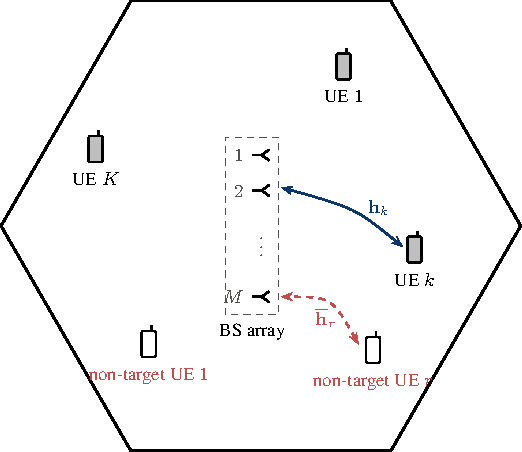
\includegraphics{Images/FLUXO/celula_interferencia.pdf}
\vspace{4pt}
\legend{Source: adapted from \citesp{marzetta2016fundamentals}, p.~32.}
\end{figure}

\subsubsection{IoTh and SNR}\label{subsec:ioth}\label{subsec:snr}
Interference over Thermal (IoTh) compares the interference power plus the thermal noise power with the thermal noise power \cite{zhao2025jsac}:
\begin{equation}
\mathrm{IoTh}=10\log_{10}\left(\frac{\beta+N_0}{\sigma^2}\right),\label{eq:iot}
\end{equation}
where $N_0=\sigma^2$ is the thermal noise power \cite{zhao2021-globecom}. The ITU-R uses the IoTh as an uplink design constraint for 5G systems, with an average value of at most 10~dB \cite{itu-m2412}. The larger the IoTh, the larger the off-diagonal elements of $\mathbf R_n$ in Equation~\ref{eq:Rn} \cite{zhao2025jsac}.
% FONTE: zhao2025jsac paper.md:577; zhao2021-globecom L207; ITU-R M.2412-0 Sec. 7.1, p. 8.

The signal-to-noise ratio (SNR) compares the energy per symbol with the thermal noise power \cite{goldsmith}:
\begin{equation}
\mathrm{SNR}=10\log_{10}\left(\frac{E_s}{\sigma^2}\right).
\label{eq:snr}
\end{equation}
The higher the SNR, the lower the symbol error probability \cite{tse-viswanath}.
% FONTE: goldsmith Sec. 6.1.1, pp. 173-174; tse-viswanath p. 53, Eq. 3.13.


% =====================================================================
\section{Equalization}\label{subsec:equalization}
% =====================================================================
Equalization estimates the symbol vector $\mathbf s$ from the received signal $\mathbf y$ by combining the signals from all antennas. \textcolor{blue}{Detection then maps each estimated symbol to a point in the constellation.}

\subsection{Maximum Likelihood Detector}\label{subsubsec:ml}
% FONTE: TG1 (sbc-template.tex), Equalization.
The optimal method for recovering transmitted symbols in MIMO systems is the
Maximum Likelihood (ML) detector \cite{wang2021tlbdinsa}. The algorithm estimates the transmitted
symbols by finding
the candidate that minimizes the Euclidean distance between the received
signal $\mathbf{y}$ and $\mathbf{H}\mathbf{s}$:

\begin{equation}
\hat{\mathbf{s}} = \underset{\mathbf{s} \in \mathcal{S}^{K}}{\arg\min}
\left\|\mathbf{y} - \mathbf{H}\mathbf{s}\right\|_2^2
\label{eq:ml}
\end{equation}
where $\mathcal{S}^{K}$ is the set of all possible combinations of
constellation symbols transmitted by the $K$ users, and
$\left\|\cdot\right\|_2^2$ denotes the sum
of the squared magnitudes of all entries of a vector (squared Euclidean norm).

\textcolor{blue}{This method yields the lowest possible bit error rate without channel coding.} However, MIMO detection is NP-hard \cite{zero-forcing}, and an exhaustive search over $\mathcal{S}^{K}$ has a complexity of $\mathcal{O}(|\mathcal{S}|^K)$, making the ML detector impractical for systems with a large number of
users or high-order modulation schemes~\cite{bello2022algorithms}.
% FONTE: wang2021tlbdinsa p. 2971.

\subsection{Filters}\label{subsec:filtros}\label{subsubsec:wiener}

A filter receives a measured signal and produces another signal at its output. In a linear filter, each output sample is a linear combination of the measurements, where the weights serve as the filter coefficients \cite{oppenheim2010wiener}.

Linear equalizers are linear filters and suboptimal alternatives to the ML detector whose
complexity is independent of the constellation scheme employed. These
techniques estimate a continuous-valued approximation $\tilde{\mathbf{s}}$
(soft-output) of $\mathbf{s}$ by applying a weight matrix $\mathbf{W}$ to
the received signal vector $\mathbf{y}$~\cite{rodriguezsanchez2020}:
\begin{equation}\label{eq:filtro}
\tilde{\mathbf s}=\mathbf W\mathbf y.
\end{equation}

The $k$-th row of $\mathbf W$ contains the weights used to estimate the symbol for UE $k$. Linear equalizers differ in the criterion used to select these weights \cite{tse-viswanath}.
% FONTE: oppenheim2010wiener p. 195, Eq. 11.1; tse-viswanath pp. 351 e 358.

\subsubsection{Zero-Forcing Equalizer}\label{subsubsec:zf}
The Zero-Forcing (ZF) equalizer aims to eliminate interference between the UEs, without considering noise \cite{tse-viswanath}. To do this, it inverts the channel: multiplying $\mathbf y$ by the inverse of $\mathbf H$ undoes the mixing of the UE signals and leaves only the corresponding UE symbol at each output. However, $\mathbf H$ is an $M \times K$ matrix, which is not square and has no inverse. \textcolor{blue}{ZF uses the pseudo-inverse of $\mathbf H$ instead, which has the same effect of separating the symbols \cite{zero-forcing}:}
% FONTE: tse-viswanath pp. 351-352 e 358.
\begin{equation}
\mathbf{W}_\text{ZF}=
\left(\mathbf{H}^H\mathbf{H}\right)^{-1}\mathbf{H}^H,
\label{eq:zf_filter}
\end{equation}
where $\mathbf{H}^H$ denotes the conjugate transpose of $\mathbf{H}$. The product $\mathbf H^H\mathbf H$ is the Gram matrix of $\mathbf H$ \cite{jeon2019}. It is square, of size $K \times K$, and it is this matrix that ZF inverts. \textcolor{blue}{Noise also passes through the filter, since it is not considered.} As a consequence, ZF amplifies the noise present at the receiver, particularly in poorly conditioned channels.
% FONTE: jeon2019 L105 (Gram matrix).

\subsubsection{LMMSE Equalizer}\label{subsubsec:lmmse}
The Linear Minimum Mean Square Error (LMMSE) equalizer addresses the ZF
limitation by explicitly accounting for the noise statistics during equalizer
design \cite{tse-viswanath}. The estimate $\tilde{\mathbf{s}}_\text{LMMSE}$ is obtained by applying the
equalization matrix to the received signal:

\begin{equation}
\tilde{\mathbf{s}}_\text{LMMSE}=
\mathbf{W}_\text{LMMSE}\mathbf{y}
\label{eq:lmmse_estimate}
\end{equation}

The weights of $\mathbf W$ are chosen according to the criterion:

\begin{equation}
\min_{\mathbf{W}}
\mathbb{E}
\left[
\left\|\mathbf{W}\mathbf{y}-\mathbf{s}\right\|_2^2
\right],
\label{eq:lmmse_opt}
\end{equation}
% FONTE: zhao2025jsac paper.md:67 (Eq. 2); haykin p. 198, Eq. 5.36.
which minimizes the mean squared error of the equalization \cite{zhao2025jsac}. This error is calculated using the expected value $\mathbb E[\cdot]$, the average value of a random variable, since the symbols and noise are random \cite{haykin}. Thus, the minimization considers the different realizations of these variables, and not just a specific observation.
The squared error includes both interference and noise. \textcolor{blue}{Therefore, LMMSE can retain some interference to reduce noise, unlike ZF \cite{tse-viswanath}.}

% FONTE: tse-viswanath p. 358.
Assuming that the channel matrix $\mathbf{H}$ is perfectly known, the
corresponding solution for the LMMSE equalizer in a centralized MIMO system
is given by~\cite{zhao2025jsac}:

\begin{equation}
\mathbf{W}_\text{LMMSE}=
\left(
\mathbf{H}^H\mathbf{R}_n^{-1}\mathbf{H}
+
\frac{1}{E_s}\mathbf{I}
\right)^{-1}
\mathbf{H}^H\mathbf{R}_n^{-1}
\label{eq:lmmse_solution}
\end{equation}
where $\mathbf{n}$ is modeled as a zero-mean random vector with covariance
matrix $\mathbf{R}_n = \mathbb{E}[\mathbf{n}\mathbf{n}^H]$ (Section~\ref{subsubsec:interferencia}), and $E_s$
denotes the average energy per transmitted symbol. \textcolor{blue}{The LMMSE approaches the ZF with low noise \cite{tse-viswanath}.}
% FONTE: tse-viswanath p. 361.

The LMMSE equalizer leads to a slight increase in computational complexity
compared with ZF, as it additionally requires estimating the noise covariance matrix $\mathbf{R}_n$ to compute the filter. Both equalizers share the same asymptotic complexity
$\mathcal{O}(K^3)$, dominated by the matrix inversion, but the LMMSE
generally achieves a lower BER than ZF~\cite{li-tradeofs}.
% FONTE: li-tradeofs Fig. 5(a).

The equalization
matrix $\mathbf{W}$ is computed only once per coherence block and reused for
each received symbol, reducing the average computational cost per symbol by a
factor of $1/N_\text{coh}$, where $N_\text{coh}$ is the number of symbols in the block \cite{zhao2025jsac}.
% FONTE: zhao2025jsac paper.md:561.

\subsubsection{BCD-MMSE Equalizer}\label{subsubsec:bcd-filtro}
% FONTE: TG1 (sbc-template.tex), BCD-MMSE Algorithm.
\textcolor{blue}{The base station in the decentralized MIMO architecture is divided into $C$ clusters, so that each cluster receives only the signals of its $M_c$ antennas and does not have knowledge of the complete channel.} The LMMSE of Equation~\ref{eq:lmmse_solution}, however, needs $\mathbf H$ and $\mathbf R_n$ of all $M$ antennas. Therefore, the equalization algorithm needs to be adapted to this architecture. The BCD-MMSE algorithm was proposed to adapt the LMMSE to the decentralized MIMO architecture, with the DUs connected in a daisy-chain \cite{zhao2025jsac}.

The BCD-MMSE algorithm partitions the global equalization matrix
$\mathbf{W} \in \mathbb{C}^{K \times M}$ into $C$ local blocks
$\mathbf{W}_c \in \mathbb{C}^{K \times M_c}$, one per DU, and minimizes
the mean squared error of Equation~\ref{eq:lmmse_opt} one block at a time \cite{zhao2021-globecom}.
To estimate $\mathbf s$, each DU multiplies its block $\mathbf W_c$ by the signal received at its antennas, $\mathbf y_c$, and the results of all DUs are summed \cite{zhao2025jsac}:
\begin{equation}\label{eq:bcd_filtro}
\tilde{\mathbf s}_{\text{BCD-MMSE}} = \sum_{c=1}^{C}\mathbf W_c\mathbf y_c.
\end{equation}
% FONTE: zhao2025jsac, Algoritmo 3, paper.md:430-434 (filtro); zhao2021-globecom (atualização por bloco).

\subsection{Detection and Symbol Error Rate}\label{subsubsec:ser}

The detector selects the constellation point closest to each entry of $\tilde{\mathbf s}$ and forms the detected vector $\hat{\mathbf s}$ \cite{zhao2025jsac}. An error occurs when the detector chooses a point different from the transmitted symbol. The Symbol Error Rate (SER) corresponds to the probability of such an error occurring. Comparing two equalizers involves examining the difference in the SNR required for both to achieve the same SER. This difference corresponds to the horizontal distance between their respective SER-versus-SNR curves at a fixed error rate. \textcolor{blue}{This work adopts an SER of $10^{-2}$ as a reference \cite{tse-viswanath,wang2021tlbdinsa}.}
% FONTE: tse-viswanath p. 503 e p. 55, nota 4; wang2021tlbdinsa L416.


% =====================================================================
\section{BCD-MMSE Computation}\label{sec:calculo-bcd}\label{sec:dbp-ruido}
% =====================================================================
This section shows how each DU calculates its BCD-MMSE block $\mathbf W_c$ (Section~\ref{subsubsec:bcd-filtro}).

% ---------------------------------------------------------------------
\subsection{Covariance Estimation}\label{subsec:rcc-local}\label{subsec:ruido-colorido}\label{subsubsec:estimacao-R}
% ---------------------------------------------------------------------
The BS knows the channel matrix $\mathbf H$ of its UEs, but it does not know the matrix $\overline{\mathbf H}$ of the non-target UEs nor the power $\beta$ with which they transmit. Therefore, the BS estimates $\mathbf R_n$ by averaging $N$ samples of noise it receives \cite{tomasin-interference}:


\begin{equation}\label{eq:Rn_est}
\widehat{\mathbf R}_n=
\frac{1}{N}
\sum_{i=1}^{N}
\mathbf n^i(\mathbf n^i)^H,
\end{equation}


where $\mathbf n^i\in\mathbb C^{M\times1}$ is the noise sample in the $i$-th pilot RE, reference REs that the UEs transmit to the BS to estimate the channel \cite{marzetta2016fundamentals}. The receiver knows the pilot of the target UEs and can remove it from the received signal. What remains is interference plus thermal noise. Each element of $\mathbf n^i(\mathbf n^i)^H$ is the product $n_a^i(n_b^i)^*$ between the noise of two antennas. The diagonal elements ($a=b$) are the power in one antenna. The average of these products estimates each element of $\mathbf R_n$. The receiver performance improves with the number of samples $N$ \cite{tomasin-interference}.
% FONTE: Marzetta et al., Seção 3.1, p. 45.
% FONTE: tomasin-interference p. 1773, Eq. 6; Figs. 5 e 6.

In the decentralized uplink, each noise sample is also divided between the clusters, $\mathbf n^i = [(\mathbf n_1^i)^T, \ldots, (\mathbf n_C^i)^T]^T$, and the DU $c$ only keeps its part. Likewise, $\mathbf R_n$ becomes \textcolor{red}{a matrix} of $C \times C$ blocks\textcolor{red}{. The block $\mathbf R_{\mathrm{row},\mathrm{col}} = \mathbb E[\mathbf n_{\mathrm{row}}\mathbf n_{\mathrm{col}}^H]$ relates the noise of the antennas of cluster $\mathrm{row}$ to the noise of the antennas of cluster $\mathrm{col}$ (Figure~\ref{fig:rn-blocos})}. Each DU can only estimate its diagonal block with its own samples \textcolor{red}{\cite{zhao2021-globecom,zhao2025jsac}}:

% FONTE: zhao2021-globecom L88 e L90.
\begin{equation}
\hat{\mathbf R}_{cc}=
\frac{1}{N}
\sum_{i=1}^{N}
\mathbf n_c^i(\mathbf n_c^i)^H.
\label{eq:Rcc_est}
\end{equation}

Off-diagonal blocks, \textcolor{red}{$\mathbf R_{\mathrm{row},\mathrm{col}}$ with $\mathrm{row} \neq \mathrm{col}$}, combine the noise from two clusters. To estimate them, the DUs would have to exchange $N$ samples for each of the $M$ antennas, which is not feasible in massive MIMO. Therefore, BCD-MMSE does not exchange samples. Each DU uses only the samples from its cluster and passes the results $\mathbf A_c$ and $\mathbf b_{c,i}$ to the next DU in the chain (\textcolor{red}{Figure~\ref{fig:bcd-etapas}(b)} and Section~\ref{subsec:bcd}). The size of these results depends on the number of UEs $K$, and not on the number of antennas $M$ \cite{zhao2025jsac}.

% FONTE: zhao2025jsac paper.md:39-41, :125, :130 e :571.

\begin{figure}[!ht]
\caption[Blocks of $\mathbf R_n$.]{Blocks of $\mathbf R_n$, with $C \times C$ blocks of $M_c \times M_c$ elements. In red, the blocks that DU 3 needs.}
\label{fig:rn-blocos}
\vspace{4pt}
\centering
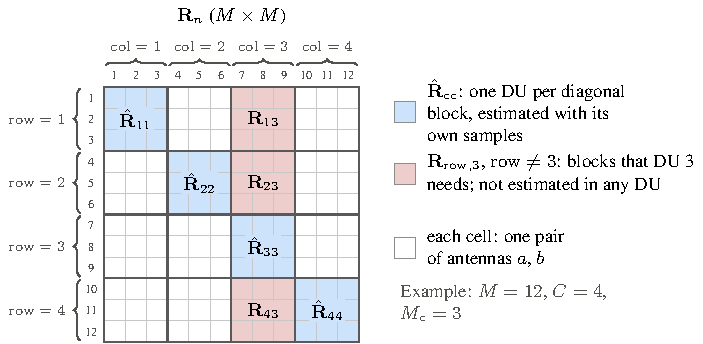
\includegraphics{Images/FLUXO/rn_blocos.pdf}
\vspace{4pt}
\legend{Source: adapted from \citesp{zhao2025jsac}.}
\end{figure}
% FONTE: zhao2025jsac, Fig. 3 (paper.md:127-128) e Algoritmo 3.

\subsubsection{Availability of Noise Samples within the Coherence Time}\label{subsubsec:disponibilidade-amostras}
All samples used in noise estimation must represent the same covariance matrix. Therefore, the sampling interval is limited by the variation in time and frequency of the channels that determine the interference. \textcolor{red}{These variations define the coherence block (Section~\ref{subsec:bloco-coerencia}). Thus, the estimate $\hat{\mathbf R}_{cc}$} is unique per PRB within each coherence time.


\textcolor{blue}{The Demodulation Reference Signal (DM-RS) in 5G NR is the reference signal (pilot) transmitted by the UE to allow the receiver to estimate channel conditions.} The DM-RS is transmitted alongside the PUSCH (Section~\ref{subsec:simbolos}) within the same PRBs. The double-symbol DM-RS occupies two consecutive OFDM symbols at each position within the slot and allows for the differentiation of up to 12 UEs \cite{3gpp-ts38211}.
% FONTE: TS 38.211 Sec. 6.4.1.1.3, Tabs. 6.4.1.1.3-2, 6.4.1.1.3-4 e 6.4.1.1.3-5.

\textcolor{red}{The receiver obtains the} noise samples from the REs occupied by the DM-RS. \textcolor{red}{Assim, só há amostras nos slots em que os UEs alvo transmitem o PUSCH.} The number of samples therefore depends on how many DM-RS REs are present within the interval over which the covariance remains constant. \textcolor{blue}{The double-symbol DM-RS occupies 4 OFDM symbols, with a maximum of two positions per slot \cite{3gpp-ts38211}.} \textcolor{red}{Thus,} each PRB \textcolor{red}{has at most} 4 $\times$ 12 = 48 DM-RS REs per slot. Figure~\ref{fig:prb-dmrs} illustrates these REs within a PRB.

\definecolor{dmrsfill}{HTML}{CDE2FB}
\definecolor{winblue}{HTML}{0D366B}
\definecolor{inksec}{HTML}{52514E}
\begin{figure}[htbp]
\caption[Resource elements of one PRB in one slot, with the DM-RS symbols.]{Resource elements of one PRB in one slot, with the DM-RS symbols. Double-symbol DM-RS, mapping type~A, symbols 2, 3, 10 and 11.}
\label{fig:prb-dmrs}
\vspace{4pt}
\centering
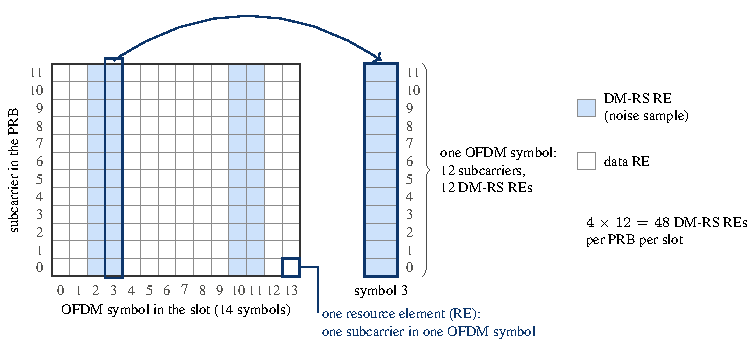
\includegraphics{Images/FLUXO/prb_dmrs.pdf}
\vspace{4pt}
\legend{Source: the author, with the DM-RS positions of \citesp{3gpp-ts38211}.}
\end{figure}


\textcolor{red}{Since the samples must fall within the same interval of duration $T_c$ as the data symbol,} the number of available samples may vary from one data symbol to another. \textcolor{blue}{The number of samples for a given symbol corresponds to the maximum count of DM-RS REs found within an interval of duration $T_c$ that encompasses that symbol.} The number of samples available for all symbols in the slot is the smallest of these values. Figure~\ref{fig:dmrs-n} shows an example with the DM-RS located at symbols 2, 3, 10, and 11 of each slot. \textcolor{red}{Symbols 5 through 8 are the worst case under the TDLB100-400 condition}, with 24 samples. Therefore, the number of samples available for all symbols is 24. Table~\ref{tab:n-maximo} presents this value for each test condition.

\begin{table}[htbp]
\caption[Number of DM-RS REs per PRB available to every data symbol of the slot, in each test condition.]{Number of DM-RS REs per PRB available to every data symbol of the slot, in each test condition. Double-symbol DM-RS in symbols 2, 3, 10 and 11, with every slot carrying PUSCH.}
\label{tab:n-maximo}
\vspace{4pt}
\centering
\footnotesize
\renewcommand{\arraystretch}{1.2}
\setlength{\aboverulesep}{0pt}
\setlength{\belowrulesep}{0pt}
\begin{tabular}{|c|c|c|c|c|}
\toprule
\multirow{2}{*}{\textbf{Test condition}} & \textbf{Frequency} & \multirow{2}{*}{{\boldmath $T_c$} \textbf{(ms)}} & \textbf{OFDM symbols} & \textbf{DM-RS REs} \\
 & \textbf{range} & & \textbf{in} {\boldmath $T_c$} & \textbf{available} \\
\midrule
TDLA30-5    & \multirow{2}{*}{FR1} & 25.0000 & 700 & 2400 \\
TDLA30-10   &                      & 12.5000 & 350 & 1200 \\
\cline{2-2}
TDLA30-75   & \multirow{2}{*}{FR2} & 1.6667  & 186 & 648 \\
TDLA30-300  &                      & 0.4167  & 46  & 168 \\
\cline{2-2}
TDLC300-100 & \multirow{4}{*}{FR1} & 1.2500  & 35  & 132 \\
TDLB100-400 &                      & 0.3125  & 8   & 24 \\
HST350      &                      & 0.0536  & \multirow{2}{*}{1} & \multirow{2}{*}{0} \\
HST500      &                      & 0.0375  &     &  \\
\bottomrule
\end{tabular}
\vspace{4pt}
\legend{Source: the author, from \citesp{3gpp-ts38104}; \citesp{3gpp-ts38211}; \citesp{tse-viswanath}.}
\end{table}

\textcolor{red}{The interval with the most DM-RS REs for a data symbol} may include DM-RS that arrive after that symbol. In Figure~\ref{fig:dmrs-n}(b), \textcolor{red}{this interval for} symbol 13 goes up to symbol 3 of the next slot. \textcolor{blue}{The receiver needs to store symbol 13 for 4 more symbols to use these samples.}
% FONTE: contagens em Python (DM-RS em {2,3,10,11}, slots contínuos, L = 8).
\definecolor{dmrsfill}{HTML}{CDE2FB}
\definecolor{winblue}{HTML}{0D366B}
\definecolor{inksec}{HTML}{52514E}
\begin{figure}[htbp]
\caption[Intervals of duration $T_c$ that contain a data symbol, and their DM-RS REs per PRB, in the TDLB100-400 condition.]{Intervals of duration $T_c$ that contain a data symbol, and their DM-RS REs per PRB, in the TDLB100-400 condition. Double-symbol DM-RS, mapping type~A, symbols 2, 3, 10 and 11; continuous uplink. In (a) and (b), each bar is one position of an interval of duration $T_c$ that contains the marked symbol. Symbol 6 is the worst case of the slot, and symbol 13 is a best case.}
\label{fig:dmrs-n}
\vspace{4pt}
\centering
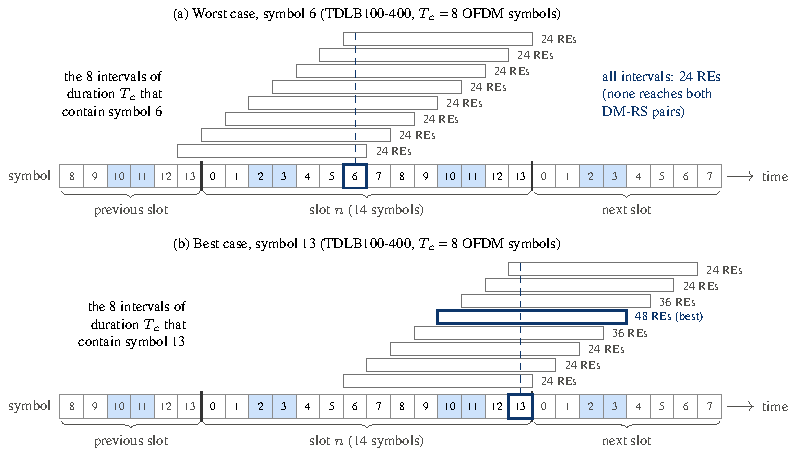
\includegraphics{Images/FLUXO/dmrs_n.pdf}
\vspace{4pt}
\legend{Source: the author, with the DM-RS positions of \citesp{3gpp-ts38211}.}
\end{figure}


\subsubsection{Conditioning of the Estimate}\label{subsubsec:condicionamento-R}


The singular values ​​of a matrix $\mathbf X$ are the square roots of the eigenvalues ​​of $\mathbf X\mathbf X^H$ and measure how much the matrix expands or reduces a vector in each direction. The rank of a matrix is ​​the number of its non-zero singular values, and measures the amount of non-redundant information in matrices. A sum of $N$ matrices of rank 1 has a rank of at most $N$ \cite{tse-viswanath}. Each term $\mathbf{n}^i(\mathbf{n}^i)^H$ of \eqref{eq:Rn_est} has rank 1, because all its columns are multiples of $\mathbf{n}^i$. Therefore:
% FONTE: Tse e Viswanath, Seção 7.1.1, pp. 291-292, Eqs. 7.2 a 7.4.

\[
\operatorname{rank}(\widehat{\mathbf R}_n) \leq \min(M,N)
\]

A matrix is ​​considered singular when its rank is strictly less than its dimension. Singular matrices do not have an inverse. Thus, $\widehat{\mathbf R}_n$ has no inverse when $N<M$, and $\hat{\mathbf R}_{cc}$ has no inverse when $N<M_c$.


The number of antennas in a massive MIMO system can exceed the number of samples in a coherence block (Table~\ref{tab:n-maximo}). Ledoit-Wolf shrinkage renders the estimate invertible. It blends $\widehat{\mathbf R}_n$ with a multiple of the identity matrix, using a weight calculated from the samples themselves \cite{ledoit-wolf}.
% FONTE: N da Tabela tab:n-maximo (24 a 2400 REs de DM-RS por PRB, 0 nos HST).
% FONTE: Ledoit e Wolf (2004). Simulador: m5_noise.shrink.

The condition number of a matrix is ​​the ratio between its largest and smallest singular values ​​\cite{tse-viswanath}. The error in matrix inversion using a low number of bits increases with the condition number, and this number is linked to the ratio of interference to noise \cite{osinsky2023}. In this work, this ratio is measured via the IoTh (Section~\ref{subsec:ioth}).
% FONTE: Tse e Viswanath, Seção 7.1.2, p. 295; Osinsky et al. 2023, p. 1603.
% FONTE: Tse e Viswanath, Seção 3.3.2, p. 75, nota 9, Eq. 3.83; Eq. 7.2, p. 292.


% ---------------------------------------------------------------------
\subsection{Algorithm Steps}\label{subsubsec:bcd-etapas}
% ---------------------------------------------------------------------
The BCD-MMSE has three phases: preprocessing, iterations, and filtering. The preprocessing calculates the initial equalizer $\mathbf W^0$ with the covariance of the block-diagonal noise, that is, each DU uses only its $\mathbf R_{cc}$ \cite{zhao2021-globecom,zhao2025jsac}:

% FONTE: zhao2021-globecom L90-94 (aproximação bloco-diagonal, Eq. 6 = W^0).
\begin{equation}\label{eq:bdac}
\mathbf W^0 = \left(\sum_{c=1}^{C}\mathbf H_c^H\mathbf R_{cc}^{-1}\mathbf H_c + \frac{1}{E_s}\mathbf I\right)^{-1}\left[\mathbf H_1^H\mathbf R_{11}^{-1}, \ldots, \mathbf H_C^H\mathbf R_{CC}^{-1}\right].
\end{equation}

Each DU calculates the matrix $K \times K$ $\mathbf H_c^H\hat{\mathbf R}_{cc}^{-1}\mathbf H_c$. The DUs sum these matrices along the chain. The last DU reverses the sum and sends the result to all DUs (Figure~\ref{fig:bcd-etapas}(a)). Each DU uses this result to calculate its block $\mathbf W_c^0$. This equalizer loses performance under colored noise, but serves as a starting point for BCD-MMSE. Finally, $\mathbf A_0^0$ is the sum of $\mathbf W_c^0\mathbf H_c$ of all DUs, and $\mathbf b_{0,i}^0$ is the sum of $\mathbf W_c^0\mathbf n_c^i$ \cite{zhao2025jsac}.

Each iteration updates the DUs in order, from $c = 1$ to $C$, by \eqref{eq:bcd_update}, \eqref{eq:A_update} and \eqref{eq:b_update}. DU 1 receives $\mathbf A_C$ and $\mathbf b_{C,i}$ from DU $C$ (Figure~\ref{fig:bcd-etapas}(b)). The algorithm can stop when the mean squared error \eqref{eq:lmmse_opt} hardly changes between two iterations. Bandwidth and computation also limit the number of iterations $T$. Two to three iterations are enough for the SER to get close to that of the centralized LMMSE, and one iteration already gives good performance \cite{zhao2025jsac}.

\begin{figure}[!ht]
\caption[BCD-MMSE initialization and iterations in the daisy chain with $C = 4$ DUs.]{BCD-MMSE initialization and iterations in the daisy chain with $C = 4$ DUs. (a) BDAC-MMSE initialization: the sums of $\mathbf X_c$ go along the chain to DU 4, which inverts the $K \times K$ matrix and sends $\mathbf P$ to all DUs. (b) Each iteration: DU $c$ receives the noise samples $\mathbf n_c^i$ of its cluster and, from the previous DU, only $\mathbf A_{c-1}$ and $\{\mathbf b_{c-1,i}\}_{i=1}^N$. DU 4 passes its results to DU 1 in the next iteration.}
\label{fig:bcd-etapas}
\vspace{4pt}
\centering
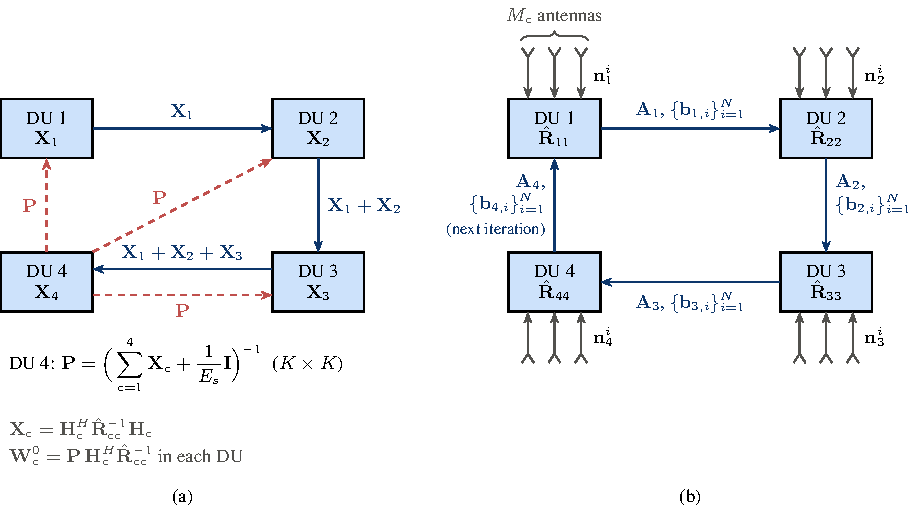
\includegraphics[width=\textwidth]{Images/FLUXO/bcd_etapas.pdf}
\vspace{4pt}
\legend{Source: adapted from \citesp{zhao2025jsac}.}
\end{figure}
% FONTE: figura de Images/FLUXO/src/bcd_etapas.tex. (a) zhao2025jsac paper.md:136-140 (Eq. 7);
%   modelo B, software/Restrições - Parâmetros.csv, linhas 56-65. (b) Algoritmo 3, paper.md:407-433 e :450.

The filter phase calculates $\tilde{\mathbf s}$ by \eqref{eq:bcd_filtro}.

% FONTE: zhao2025jsac paper.md: Eq. 7, :132-140; Algoritmo 3, :407-433; nota 6, :450; iterações, :449, :461 e :585.
%   Inversão K x K na última DU: software/Restrições - Parâmetros.csv, linhas 56-65 (modelo B).




% ---------------------------------------------------------------------
\subsection{Block Update}\label{subsec:bcd}
% ---------------------------------------------------------------------
DU $c$ updates its block in iteration $\mathrm{iter}$ as~\cite{zhao2021-globecom,zhao2025jsac}:
% FONTE: zhao2021-globecom L152 (Eq. 8, mesma inversa (E_s H_c H_c^H + R_cc)^-1).
\begin{multline}
  \mathbf{W}_c^{\mathrm{iter}} = \left(
    E_s \left(\mathbf{I}_K - \mathbf{A}_{c-1}^{\mathrm{iter}}
    + \mathbf{W}_c^{\mathrm{iter}-1}\mathbf{H}_c\right)\mathbf{H}_c^H
    - \frac{1}{N}\sum_{i=1}^{N}
      \left(\mathbf{b}_{c-1,i}^{\mathrm{iter}} - \mathbf{W}_c^{\mathrm{iter}-1}\mathbf{n}_c^i\right)
      \left(\mathbf{n}_c^i\right)^H
  \right) \\
  \times
  \underbrace{
    \left(E_s \mathbf{H}_c \mathbf{H}_c^H
    + \hat{\mathbf{R}}_{cc}\right)^{-1}
  }_{\text{local } M_c \times M_c \text{ inversion}},
  \label{eq:bcd_update}
\end{multline}
where $\mathbf{A}_{c-1}^{\mathrm{iter}} \in \mathbb{C}^{K \times K}$ and
$\{\mathbf{b}_{c-1,i}^{\mathrm{iter}} \in \mathbb{C}^{K \times 1}\}_{i=1}^{N}$
are interaction variables received from the previous DU, and
$\hat{\mathbf{R}}_{cc}$ is given by~\eqref{eq:Rcc_est}. After updating $\mathbf{W}_c^{\mathrm{iter}}$,
DU $c$ computes the updated interaction variables
\begin{align}
  \mathbf{A}_c^{\mathrm{iter}} &= \mathbf{A}_{c-1}^{\mathrm{iter}}
    - \mathbf{W}_c^{\mathrm{iter}-1}\mathbf{H}_c
    + \mathbf{W}_c^{\mathrm{iter}}\mathbf{H}_c, \label{eq:A_update} \\
  \mathbf{b}_{c,i}^{\mathrm{iter}} &= \mathbf{b}_{c-1,i}^{\mathrm{iter}}
    - \mathbf{W}_c^{\mathrm{iter}-1}\mathbf{n}_c^i
    + \mathbf{W}_c^{\mathrm{iter}}\mathbf{n}_c^i, \quad i = 1,\ldots,N,
  \label{eq:b_update}
\end{align}
and forwards them to DU $c+1$~\cite{zhao2025jsac}.

By~\eqref{eq:b_update}, $\mathbf b_{c,i}$ is the sum of $\mathbf W_j\mathbf n_j^i$ over all DUs $j$, where $\mathbf n_j^i$ is the $i$-th noise sample of cluster $j$. In the average of~\eqref{eq:bcd_update}, each term $\mathbf W_j\mathbf n_j^i(\mathbf n_c^i)^H$ results in $\mathbf W_j\hat{\mathbf R}_{jc}$. Thus, DU $c$ uses the off-diagonal blocks without estimating them (Figure~\ref{fig:rn-blocos}) \cite{zhao2025jsac}.
% FONTE: zhao2025jsac paper.md:447; Algoritmo 3 (b_0^0) e Eq. eq:b_update.
% FONTE (conta): (1/N) sum_i W_j n_j^i (n_c^i)^H = W_j R_jc.

$\mathbf G_c$ is the matrix inverted in~\eqref{eq:bcd_update}:
\begin{equation}\label{eq:Gc}
\mathbf G_c=
E_s\mathbf H_c\mathbf H_c^H+
\hat{\mathbf R}_{cc}.
\end{equation}
$\mathbf G_c$ does not depend on the iteration $\mathrm{iter}$ \cite{zhao2025jsac}. Thus, the DU inverts $\mathbf G_c$ once per coherence block and uses the inverse in all iterations.
% FONTE: Eq. 30, paper.md:504 (G_c sem índice de iteração).

% ---------------------------------------------------------------------
\subsection{Complexity}\label{subsubsec:bcd-complexidade}
% ---------------------------------------------------------------------

Preprocessing costs $\mathcal{O}(M_c^3 + N M_c^2)$ in each DU. Each iteration costs $\mathcal{O}(NMK + M M_c K)$ summed over all DUs \cite{zhao2025jsac}. The matrices of the algorithm have complex entries. Table~\ref{tab:bcd-complexidade} gives, for each part, the number of products between two complex numbers, called complex multiplications. Several parts depend on $N$, which changes with the test condition (Table~\ref{tab:n-maximo}).

\begin{table}[htbp]
\caption{Complex multiplications per PRB and per $T_c$ in each DU.}
\label{tab:bcd-complexidade}
\vspace{4pt}
\centering
\footnotesize
\renewcommand{\arraystretch}{1.2}
\setlength{\aboverulesep}{0pt}
\setlength{\belowrulesep}{0pt}
\begin{tabular}{|l|l|}
\toprule
\textbf{Part} & \textbf{Complex multiplications} \\
\midrule
Estimate $\hat{\mathbf R}_{cc}$ and apply Ledoit-Wolf & $N M_c^2 + N M_c + M_c^2$ \\
\hline
Initialization, including the inverse of $\hat{\mathbf R}_{cc}$ & $M_c^3 + M_c^2 K + M_c K^2 + 2K^2 M_c + N K M_c$ \\
\hline
Form $\mathbf G_c$ & $M_c^2 K$ \\
\hline
Invert $\mathbf G_c$ & $M_c^3$ \\
\hline
Each iteration & $2NKM_c + 3K^2 M_c + K M_c^2$ \\
\hline
Invert the $K \times K$ matrix (DU $C$ only) & $K^3$ \\
\hline
Filter, per data symbol & $12 K M_c$ \\
\bottomrule
\end{tabular}
\vspace{4pt}
\legend{Source: the author, from \citesp{zhao2025jsac}.}
\end{table}
% FONTE: software/Restrições - Parâmetros.csv, linhas 56-65 (modelo B); zhao2025jsac paper.md:136-142,
%   :410-418, :430-434, :443-449, :504, :554 e :556.

% ---------------------------------------------------------------------
\subsection{Matrix Inversion by Cholesky Decomposition}\label{subsec:inversao}\label{sec:inversao}
% ---------------------------------------------------------------------
This work inverts $\mathbf A = \mathbf G_c$ \eqref{eq:Gc} using the Cholesky decomposition. The matrix $\mathbf A \in \mathbb{C}^{M_c \times M_c}$ is positive definite Hermitian. A square complex matrix is ​​Hermitian when it is equal to its conjugate transpose, that is, $\mathbf A^H = \mathbf A$ \cite{tse-viswanath}. A positive definite Hermitian matrix has all real and positive eigenvalues ​​\cite{wang2021tlbdinsa}. The Cholesky decomposition applies to these matrices \cite{wang2023bdnsepa} and gives the exact result \cite{li-tradeofs}. It factors $\mathbf A = \mathbf F\mathbf F^H$, where $\mathbf F$ is lower triangular, that is, it has zeros above the main diagonal \cite{li-tradeofs}.
% FONTE: TG1 (sbc-template.tex), Matrix Inversion Techniques.
% FONTE: Tse e Viswanath, Seção 3.3.2, p. 75, nota 9; wang2021tlbdinsa L625.
% FONTE: wang2023bdnsepa L250.
% FONTE: li-tradeofs L131.

The accelerator calculates the inverse explicitly. DU inverts $\mathbf G_c$ once and uses the inverse in all iterations (Section~\ref{subsec:bcd}) \cite{li-tradeofs}. After factoring, direct substitution solves $\mathbf F\mathbf F^{-1} = \mathbf I$ and gives $\mathbf F^{-1}$. The inverse is then $\mathbf A^{-1} = \mathbf F^{-H}\mathbf F^{-1}$, which only has multiplications and additions \cite{wang2021tlbdinsa}. The triangular structure of $\mathbf F$ fits into a systolic arrangement, which facilitates implementation on an FPGA \cite{wang2023bdnsepa}.
% FONTE: li-tradeofs L123; zhao2025jsac paper.md:504 (Eq. eq:Gc).
% FONTE: wang2021tlbdinsa L485.
% FONTE: wang2023bdnsepa L502.


% =====================================================================
\section{Simulators}\label{sec:simuladores}
% =====================================================================
\subsection{Channel Models for Simulation}
\label{sec:modelo-canal}
Evaluating a massive MIMO system requires a model that represents the channel while capturing the key characteristics of an array with a large number of antennas. Such a model must account for the antenna array geometry, the spatial correlation between the channel responses of different antennas, and the physical characteristics of the environment—such as the locations and orientations of base stations (BSs) and user equipment (UEs) \cite{bjornson-mimo}.

\subsubsection{Types of Channel Models}
There are two main types of channel models: deterministic and stochastic. A deterministic model always yields the same result under identical conditions, as it relies on a specific environment with fixed parameters—such as the locations of transmitters, receivers, signal scatterers, and reflectors. Examples include ray-tracing and empirical, field-based channel measurements. A drawback of this approach is that reproducing results often requires access to specific channel measurement data or 3D building models, which are not always available \cite{bjornson-mimo}.

Stochastic models are independent of any particular environment and generalize channel behavior based on selected statistical properties. They are divided into three categories \cite{bjornson-mimo}:

\begin{itemize}
\item Correlation-based: Channel responses follow a zero-mean Gaussian distribution, defined via correlation matrices. One example is the correlated Rayleigh fading model, which assumes frequency-flat fading—meaning all multipath components arrive at the antenna with the same delay. This model is sufficient for analysis within a coherence block (Section~\ref{subsec:bloco-coerencia}). 
\item Parametric: These models define statistical distributions for the number of scatterers, delays, powers, and angles of arrival/departure (AoA/AoD). They do not account for the environment's geometry and, therefore, do not cover the analysis of the channel's temporal evolution resulting from UE movement. 
\item Geometry-based: These models strike a balance between the characteristics of stochastic and deterministic models. They define a spatial distribution for the physical locations of signal scatterers surrounding transmitters and receivers and, based on this, model the channel's propagation paths in a quasi-deterministic manner. A quasi-deterministic model defines a process governed by fixed laws, yet one that incorporates a degree of randomness through noise and/or variability.
\end{itemize}

% FONTE: Björnson, Hoydis e Sanguinetti 2017, Seção 7.3, pp. 329-331 (Fig. 7.10).

\subsection{3GPP Model and QuaDRiGa Simulator}

Line of Sight (LoS) refers to an obstacle-free path that allows for a direct view between two points. Representing propagation paths solely as a line of sight is not realistic. The 3GPP has defined a geometry-based stochastic model for MIMO systems, which accounts for a combination of both Line of Sight (LoS) and Non-Line of Sight (NLoS) propagation paths. This model integrates a deterministic layout of the MIMO system, including the locations of base stations (BS) and user equipment (UE), antenna orientation, the angular dependence of transmitted or received radio wave intensity, and subcarrier frequencies, with a set of large-scale random parameters derived from statistical distributions based on channel measurements. The open-source channel simulator QuaDRiGa (Quasi-Deterministic Radio Channel Generator) implements the 3GPP 3D MIMO model \cite{bjornson-mimo} and is the simulator employed in this work.
% FONTE: Björnson, Hoydis e Sanguinetti 2017, pp. 340-342 (Seção 7.3.3, modelo 3GPP 3D e QuaDRiGa).

A propagation scenario describes a set of statistical parameters for a specific type of environment. This work employs the scenarios defined in 3GPP NR (TR 38.901) \cite{3gpp-tr38901}. Each scenario in the model is defined by a configuration file \cite{quadriga-manual}.
% FONTE: quadriga-manual p. 7.
% FONTE: quadriga-manual p. 108, Tab. 21.


% =====================================================================
\section{FPGA Implementation}\label{sec:fpga}
% =====================================================================
% ---------------------------------------------------------------------
\subsection{FPGA and the Alveo U50 Board}\label{subsec:fpga}\label{subsec:alveo-u50}
% ---------------------------------------------------------------------
An FPGA (Field-Programmable Gate Array) has programmable logic, made of lookup tables (LUTs) and flip-flops (FFs), and fixed blocks. The DSP block performs multiplications and additions, and the BRAM (Block RAM) is a memory inside the chip \cite{kastner-hls}. This work measures the resources of a circuit by the number of LUTs, FFs, DSPs and BRAMs it uses.

The Alveo U50 is an accelerator card for data centers. Its FPGA, the XCU50, has 872K LUTs, 1,743K FFs, 5,952 DSPs and 1,344 BRAMs of 36~Kb \cite{ds965}. The number of LUTs of the XCU50 is in the middle of the UltraScale+ family \cite{xmp103}.
% FONTE: Kastner et al. 2018, pp. 13-14 e 17.
% FONTE: DS965 v1.8, pp. 1-2 (Tabela 1); XMP103 v1.17, pp. 2-4.
% FONTE (conta): XMP103, 11 dispositivos com menos LUTs que o XCU50, 2 iguais e 8 com mais.

% ---------------------------------------------------------------------
\subsection{High-Level Synthesis}\label{subsec:hls}
% ---------------------------------------------------------------------
High-level synthesis (HLS) starts from a description of the circuit behavior in C or C++ and creates the RTL (Register-Transfer Level) design in Verilog or VHDL. The HLS tool decides which operations run in parallel, where to insert registers to reach the clock frequency, and how to store the data in memory. Logic synthesis then translates the RTL into a netlist of FPGA elements, and placement and routing map each element to a resource of the device \cite{kastner-hls}. Directives (pragmas) guide the HLS decisions, for example the pipelining of loops \cite{ug1399}.
% FONTE: Kastner et al. 2018, pp. 11-13; UG1399, pp. 13-14.

This work also uses loop unrolling and array partitioning. The \texttt{unroll} directive creates several copies of the loop body, which can run in parallel. The copies need to read their data in the same cycle, but a BRAM allows few accesses per cycle. The \texttt{array\_partition} directive divides the array into smaller memories, which the circuit accesses at the same time. The \texttt{cyclic} type distributes the elements among the memories in turn, and the \texttt{complete} type stores each element in FFs \cite{kastner-hls}.
% FONTE: Kastner et al. 2018, p. 41 e pp. 88-90.

% ---------------------------------------------------------------------
\subsection{Static and Dynamic Power}\label{subsec:potencia}
% ---------------------------------------------------------------------
The total on-chip power is the sum of the static power and the design power. The static power comes from the leakage current of the transistors. The design power is the dynamic power, caused by the activity of the circuit. Vivado can estimate the power from the signal activity recorded in a simulation and stored in a SAIF (Switching Activity Interchange Format) file \cite{ug907}.

An average power $P$ held for a time $t$ consumes the energy
\begin{equation}\label{eq:energia}
E = P\, t.
\end{equation}
A circuit with more power can consume less energy per task if it finishes the task in less time.
% FONTE (conta): E = P t.
% FONTE: UG907 v2022.2, pp. 6 e 21.

\subsection{Fixed-Point Representation}\label{subsubsec:ponto-fixo}
The Vitis HLS type \texttt{ap\_fixed}$\langle W, I\rangle$ represents a fixed-point number with $W$ bits in total. The integer part has $I$ bits \cite{kastner-hls}, and the fractional part has $F = W - I$ bits. This work writes the format as $\langle W, I\rangle$.

An overflow occurs when a value does not fit in the integer part. A value that does not fit in the fractional part must be rounded \cite{kastner-hls}. The \texttt{ap\_fixed} type has 7 quantization modes and 5 overflow modes, which gives 35 combinations \cite{ug1399}. Table~\ref{tab:modos-apfixed} describes each mode.

\begin{table}[htbp]
\caption{Quantization and overflow modes of the \texttt{ap\_fixed} type.}
\label{tab:modos-apfixed}
\centering
\footnotesize
\begin{tabular}{p{2.6cm}p{11cm}}
\toprule
\textbf{Mode} & \textbf{Behavior} \\
\midrule
\multicolumn{2}{l}{\textit{Quantization (affects the fractional bits)}} \\
\texttt{AP\_TRN}       & Discards the least significant bits. Rounds toward $-\infty$. \\
\texttt{AP\_TRN\_ZERO} & Rounds toward zero. For positive numbers, it is equal to \texttt{AP\_TRN}. \\
\texttt{AP\_RND}       & Rounds to the nearest value. On a tie, rounds toward $+\infty$. \\
\texttt{AP\_RND\_ZERO} & Rounds to the nearest value. On a tie, rounds toward zero. \\
\texttt{AP\_RND\_MIN\_INF} & Rounds to the nearest value. On a tie, rounds toward $-\infty$. \\
\texttt{AP\_RND\_INF}  & Rounds to the nearest value. On a tie, rounds away from zero. \\
\texttt{AP\_RND\_CONV} & Rounds to the nearest value. On a tie, rounds to the even value. \\
\midrule
\multicolumn{2}{l}{\textit{Overflow (affects the integer bits)}} \\
\texttt{AP\_SAT}       & Saturates at the largest or the smallest representable value. \\
\texttt{AP\_SAT\_ZERO} & Sets the result to zero on overflow. \\
\texttt{AP\_SAT\_SYM}  & Saturates symmetrically: the positive and negative limits have the same magnitude. \\
\texttt{AP\_WRAP}      & Discards the most significant bits that do not fit (two's complement wraparound). \\
\texttt{AP\_WRAP\_SM}  & Discards the same bits, but in sign-magnitude. \\
\bottomrule
\end{tabular}
\legend{Source: \citesp{ug1399}.}
\end{table}
% FONTE: UG1399, pp. 994-995 e 1039-1044.
% FONTE: Kastner et al. 2018, pp. 70-71 (estouro e arredondamento), pp. 73-74 (ap_fixed<W, I>).

\subsection{Latency, Interval and Throughput}\label{subsubsec:latencia-intervalo}
In HLS, a task is a function call. The task latency is the time from the start to the end of a task. The task interval is the time from the start of one task to the start of the next one. A pipelined circuit can start a new task before the previous one ends, so the interval can be smaller than the latency. Many tools call the interval throughput. A larger interval means fewer tasks per unit of time, that is, a lower throughput. The initiation interval (II) is the interval between two data items that enter the pipeline.

In a sequence of tasks, the first task ends after the latency $L$, and each of the next tasks ends one interval $I$ after the previous one \cite{kastner-hls}. So, $n$ tasks end at
\begin{equation}\label{eq:fim-tarefas}
t_n = L + (n-1)\, I.
\end{equation}
\textcolor{blue}{A task in this work is one matrix inversion, and the throughput is measured by the interval between inversions.}
% FONTE: Kastner et al. 2018, pp. 20-22 (Fig. 1.7) e p. 45.

\subsection{Task Pipeline}\label{subsubsec:pipeline-tarefas}
A task can have several steps. \textcolor{blue}{The steps of a task pipeline work at the same time, each one on different data.} So, the next task starts when the previous one finishes the first step. The interval of the whole pipeline is never smaller than the interval of the slowest step \cite{kastner-hls}. \textcolor{blue}{The \texttt{dataflow} directive in HLS creates this pipeline and lets functions and loops overlap \cite{ug1399}.}
% FONTE: UG1399, pp. 787-788 (DATAFLOW) e 855-856 (UNROLL).
% FONTE: Kastner et al. 2018, pp. 113-115.

\subsection{Systolic Array}\label{subsubsec:arranjo-sistolico}
A systolic array is a set of identical processing elements (PEs), in which each PE exchanges data only with its neighbors. Unrolling an inner loop can create this kind of design, with each copy of the loop body as one PE \cite{kastner-hls}.
% FONTE: Kastner et al. 2018, pp. 153 e 180, glossário.

Figure~\ref{fig:sistolico-classico} shows a grid systolic array that computes the Gram matrix of $\mathbf H$. This matrix is Hermitian, so the array computes only the lower triangle. The array reads one row of $\mathbf H$ per cycle. The data enter from the top and from the left and move to the PE below and to the PE on the right. Each PE multiplies its two inputs and accumulates the product. After all rows are read, each PE holds one element of the matrix \cite{wang2021tlbdinsa}.
% FONTE: wang2021tlbdinsa p. 2979, Fig. 14.

\begin{figure}[!ht]
\caption[Lower triangular systolic array that computes a Gram matrix.]{Lower triangular systolic array that computes a Gram matrix. $a_j$ and $b_i$: elements of one row of $\mathbf H$.}
\label{fig:sistolico-classico}
\vspace{4pt}
\centering
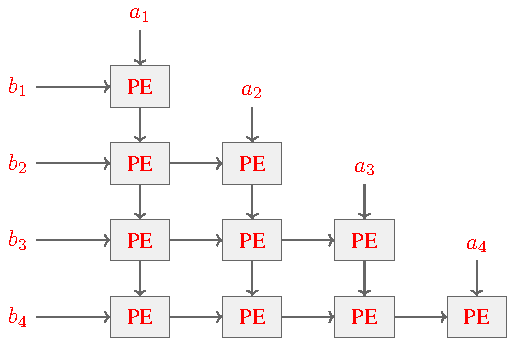
\includegraphics{Images/FLUXO/inversao_cholesky.pdf}
\vspace{4pt}
\legend{Source: adapted from \citesp{wang2021tlbdinsa}.}
\end{figure}

